\documentclass[landscape]{report}
\title{CMSI 488 Homework 1}
\author{Don Rowe}
\date{Due February 21, 2012}

\usepackage{listings}
\usepackage[landscape]{geometry}
\usepackage{graphicx}

\lstset{
  basicstyle=\footnotesize
}

\begin{document}

  \maketitle
  
  \begin{enumerate}
    \item %1
    \begin{enumerate}
      \item %1a
        \lstinputlisting{src/prob1a.regex}
        Canadian postal are in the format A0A 0A0, where ``A" is any English
        capital except for D, F, I, O, Q, or U and ``0" is any digit.
        Additionally, the first letter cannot be W or Z. Also, notice the
        space between the groups of three.
      \item %1b
        \lstinputlisting{src/prob1b.regex}
        Visa card numbers begin with a 4 and are followed by either 12 or 15
        more digits. The above regular expression assumes that there are always
        at least the first 13 digits with an optional additional 3 digits.
      \item %1c
        \lstinputlisting{src/prob1c.regex}
        MasterCard numbers begin with a 5, and the second digit is between 1
        and 5. The remaining 14 digits can be any digit.
      \item %1d
        \lstinputlisting{src/prob1d.regex}
        Numeric literals in Ada95 come in two flavors: based literals and
        decimal literals.
        
        A based literal is separated into three sections
        delimited by \# signs. The first section is any number of digits,
        possibly separated at arbitrary intervals after the first digit by an
        underscore character; this sequence, represented by
        \lstinline`\d+(_\d+)*` in the regular expression, is simply called a
        numeral. The second section is a based numeral possibly having a
        fractional part after a dot; based numerals are like numerals, only
        they are hexadecimal and are represented by
        \lstinline`[\dA-F](_[\dA-F]+)*` in the regular expression. The third
        section is an optional exponent notated with a capital E, an optional
        plus or minus sign, and a numeral; an exponent is represented in the
        regular expression by \lstinline`(E[\+\-]?\d+(_\d)*)`.
        
        A decimal literal is comprised of a numeral followed by an optional
        fractional part and an optional exponent.
      \item %1e
        \lstinputlisting{src/prob1e.regex}
        This language includes strings made up of any combination of the
        characters ``a", ``b", and ``c", provided ``a" is never followed
        immediately by another ``a" (represented in the regular expression by
        \lstinline`a(?!a)`) and provided ``b" is never followed immediately by
        ``ab" (represented by \lstinline`b(?!ab)`). To ensure that the pattern
        is applied to the whole string, the beginning \^ and ending \$ are
        included in the regex; otherwise, legal substrings of an illegal string
        can be matched. For example, the string accccbabaaccccbcbba does not
        match as a whole, but the substrings acccc, ab, and accccbcbba (split
        by the first b and third a) are matched.
    \end{enumerate}
    \item %2
      \lstinputlisting{src/prob2.js}
    \item %3
    \begin{enumerate}
      \item %3a
        This grammar produces strings made of the characters ``a" and ``b".
        The shortest string in this language is ``a": if a string begins with a
        ``b", it must be followed by at least ``aa". If a string in this
        language ends with a ``b", it must be immediately preceded by an ``a".
      \item %3b
        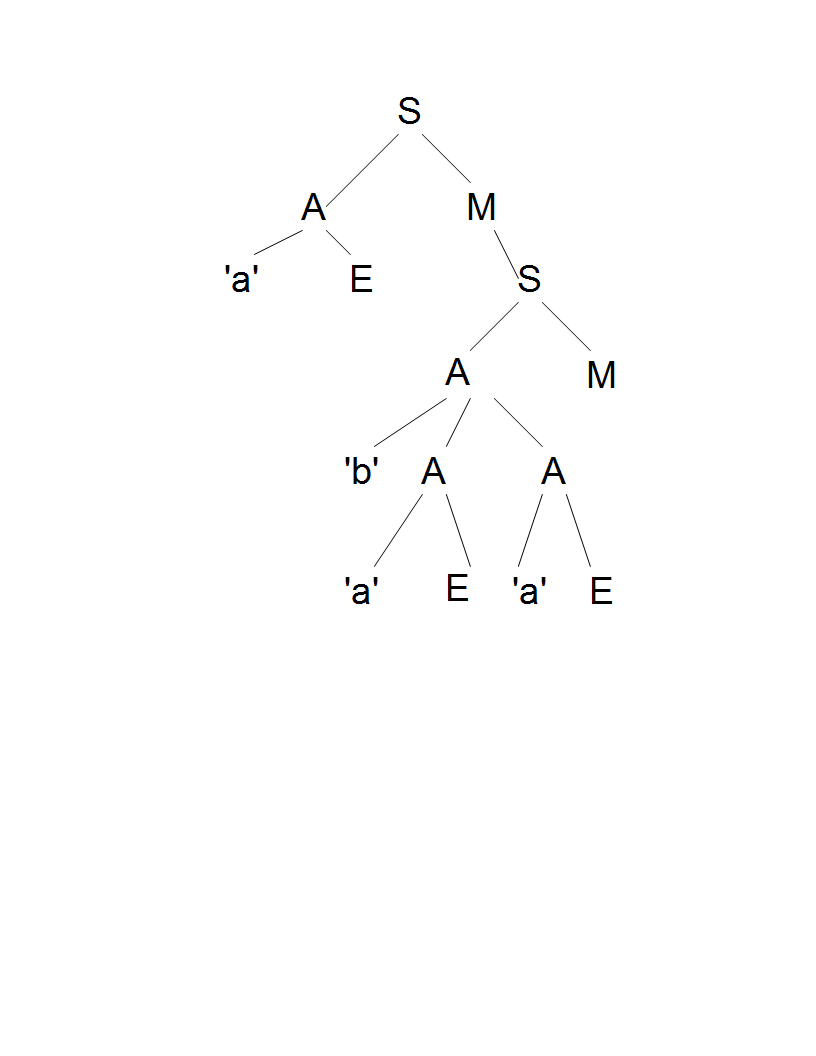
\includegraphics{img/prob3b.png}
      \item %3c
        At every choice point of this grammar, the first token of one choice is
        always `a' and the first token of the second choice is always `b'. Thus
        one only need look forward one token to determine which choice was
        made. Therefore, this grammar is LL(1).
      \item %3d
        Grammars are ambiguous if there exists a string for which there is more
        than one way to parse it. Below is another parse tree for ``abaa".
        Therefore, this grammar is ambiguous.
        
        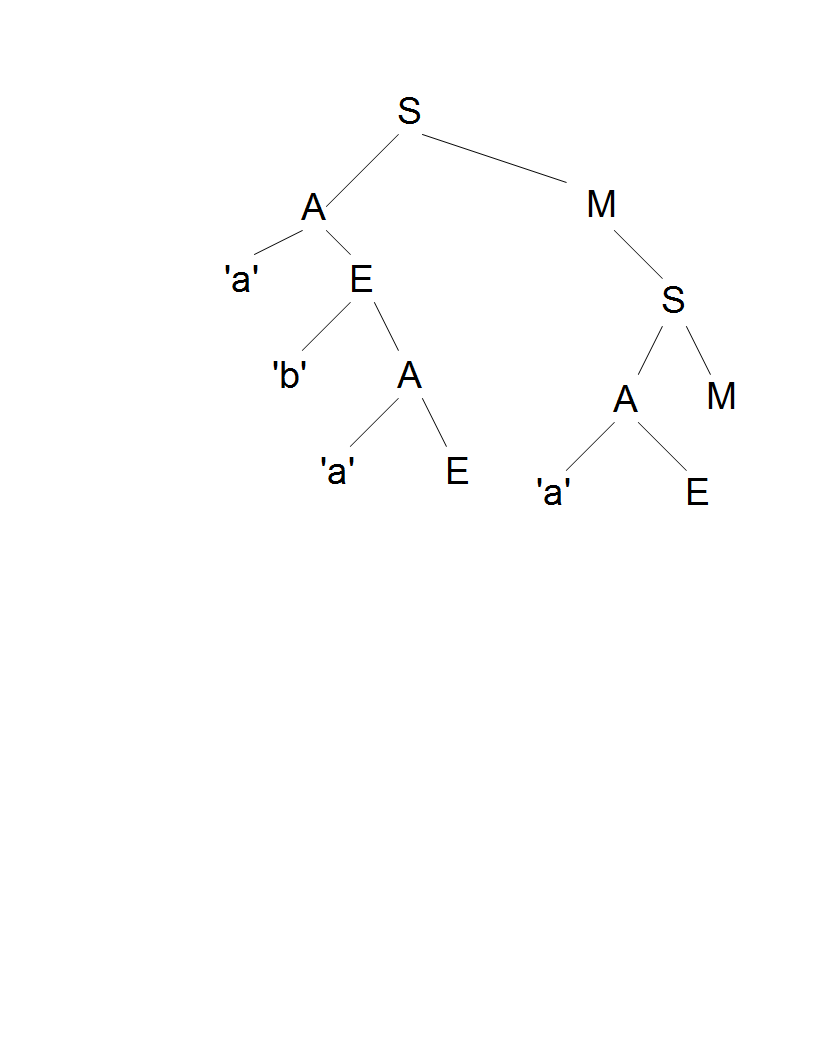
\includegraphics{img/prob3d.png}
    \end{enumerate}
    \item %4
    \begin{enumerate}
      \item %4a
        At the rule \em EXP \em lies a choice point with two choices: 
        \em ID ``:=" EXP \em and \em TERM TERM\_TAIL \em. \em TERM \em expands
        to \em FACTOR FACTOR\_TAIL \em, and \em FACTOR \em expands to \em ``("
        EXP ``)" | ID \em. Thus, in \em EXP \em's choice point, both choices
        can begin with an \em ID \em token, so by looking only one token
        forward always, one cannot be sure which choice was taken by the
        generator. Therefore, this grammar is not LL(1).
      \item %4b
        \lstinputlisting{src/prob4b.gram}
    \end{enumerate}
    \item %5
      The unary negation operator was placed with the ADDOPs for symmetry--
      indeed, unary negation in the form of $-x$ is an implication of $0-x$.
      Additionally, since $y--x$ (that is, subtracting $-x$ from $y$) cannot
      occur in Ada, it is consistent to throw out any case of an operator
      immediately preceding a unary negation operator.
      
      The expression \lstinline{-8 * 5} can be thus represented with this
      abstract syntax tree:
      
      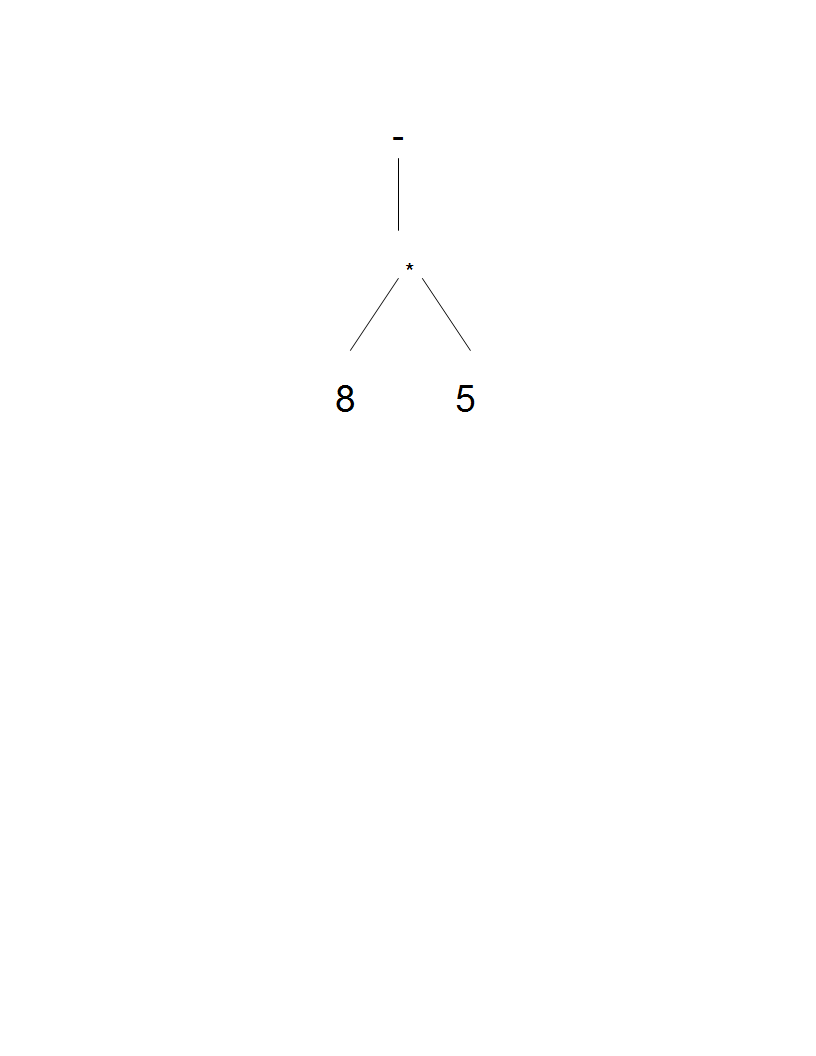
\includegraphics{img/prob5.png}
      
      This parsing is similar to parsing with the negation operator in EXP4 in
      that the answer is still -40 since the negation operator is commutative.
      The parsing is different, though, in that the negation is applied to the
      whole product of $8 * 5$ as opposed to applying the negation first to 8.
    \item %6
      
  \end{enumerate}

\end{document}
